
\externaldocument{Problem}
\section{Resource Dominated Circuit}

Scheduled sequencing graph $G_{s}(V, E) $ will be used in this section without the source and sink vertices ($ v_{0},v_{n} $). So,$\{v_{i}, i = 1, 2, ... ,n\} $. 



$ E=\{\{v_{i},v_{j} $ and $ ((t_{i}+d_{i}\leq t_{j}) $ or $ (t_{j}+d_{j}\leq t_{i})),i,j=1,2,...,n_{ops}\} $
$ \{((t_{i}+d_{i}\leq t_{j}) $ or $ (t_{j}+d_{j}\leq t_{i})),i,j=1,2,...,n_{ops}\}$
$ \tau(v_{1})= multiplier $

\subsection{Resource sharing and binding in Non-Hierarchical sequence graph}

As explain before two or more operation can be bound to the same resource. Before we bond them together we need to ensure that they are \textit{compatible}. Two conditions that the operations should met in order to be \textit{compatible} :

\begin{itemize}
\item The operations is not concurrent.
\item The operations can be implemented by resources of the same type.
\end{itemize}

So, $ E+\{(v_{i},v_{j})|\tau(v_{i}=v_{j} $ and $ ((t_{i}=d_{i} \leq t_{j}) $ or $ t_{j}=d{j} \leq t_{i})),i,j=1,...,n_{ops}\}$ %%where,

%$ \tau(v_{i}), i = 1,2,...,n_{ops} $

%$ T=\{t_{i};i=1,2,...,n_ops\} $

%$ D=\{d_{i}; i = 1,2,...,n_{ops}\} $

%$ t_{i}$

%$ t_{i}+d_{i}-1 $

The compatibility can be analyzed using compatibility graph, conflict graph and conflict graph as interval.




\subsubsection{ILP model for solving binding problem}
$ B=\{b_{ir};i=1,2,...,n_{pos};r=1,2,...,a\} $
$ X=\{x_{il};i=1,2,...,n_{pos};l=1,2,...,\lambda+1\} $
$ a\leq n_{ops} $
$ \beta(v_{i})=(1,r) $
$ l = t{i} $
$$ \sum_{r=1}^{a} b_{ir} = 1, i=1,2,...,n_{ops} $$
$$ \sum_{i=1}^{n_{ops}} b_{ir}\sum_{m=l-d_{i}+1}^{l} x_{im} \leq 1, l=1,2,...,\lambda + 1, r=1,2,...,a $$
$$ b_{ir} \in \{0,1\}, 1 =1,2,...,n_{ops}, r=1,2,...,a $$


$ \sum_{r=1}^{a_{1}} b_{ir} = 1,\forall_{i} : \tau(v_{i})=1 $
$ \sum_{i=:\tau(v_{i})=1}^{} b_{ir} x_{il} \leq 1, l=1,2,...,\lambda + 1, r=1,2,...,a_{1}$

$ \sum_{r=1}^{a_{2}} b_{ir} = 1,\forall_{i} : \tau(v_{i})=2$
$ \sum_{i=:\tau(v_{i})=2}^{} b_{ir} x_{il} \leq 1, l=1,2,...,\lambda + 1, r=1,2,...,a_{2}$

$ b_{i1} = 1, \forall_{i} \in \{1,2,3,6,7,8\} $
$ \sum_{i\in \{1,2,3,6,7,8\}}^{} b_{i1} x_{il} \leq 1, l=1,2,...,5$

$ b_{i1}=b_{i2} = 1, \forall_{i} \in \{1,2,3,6,7,8\} $
$ \sum_{i\in \{1,2,3,6,7,8\}}^{} b_{i1} x_{il} \leq 1, l=1,2,...,5$
$ \sum_{i\in \{1,2,3,6,7,8\}}^{} b_{i2} x_{il} \leq 1, l=1,2,...,5$


\ref{fig:tabu}
\begin{figure}[h]
    \centering
    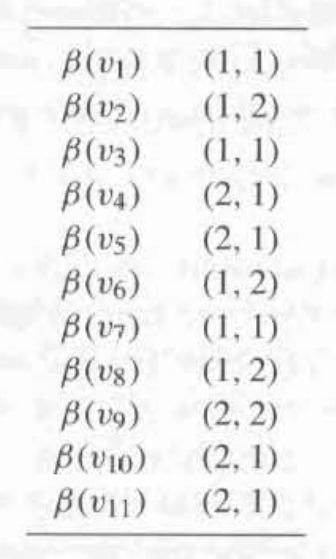
\includegraphics[width=0.18\textwidth]{tabu}
    \caption{ Tne tabulation of the binding \cite{b1}}
    \label{fig:tabu}
\end{figure}






	
%	non hierarchical sequence graph
%		compatibility graph
%			equation
%			model
%		conflict graph
%			complement of compatibility graph
%			model(vertex color)
%			clique
%		conflict graph as an interval
%			execution interval
%			intersection between two interval
%			minimum vertex coloring in polynomial time
%		
%	resource sharing and binding in sequence graph
%		model call
%			single call
%			multiple call
%		iteration
%			unroll
%			similar to model call
%		branching
		
	


